\section{Serialization}
\label{serialization}

This section is about representing objects as a sequence of bytes. We will call this sequence \textit{stream}, its formal Type will be named $S$, the current stream will be named $s$. We will assume that there is an implicit conversion between fixed sized integers\footnote{As well as between fixed sized floating point numbers, because we define them to be IEEE-754 encoded 32-/64-bit sequences.} and streams. We also make use of a stream concatenation operator $\circ : S \times S → S$.

This section assumes, that all objects about to be serialized are already known. It further assumes, that their types and thus the values of the functions (i.e. baseTypeName, typeName, index, $\den{\_}$) explained below can be easily computed.

The serialization function $\den{\_}_\tau : \tau \times \mathcal{T} → S$ will be written simply as \den{\_} if $\tau$ is clear form the context.


\subsection{Steps of the Serialization Process}

In general it is assumed that the serialization process is split into the following steps:
\begin{enumerate}
 \item All objects to be serialized are collected. This is usually done using the transitive closure of an initial set.
 
 \item The items are organized into their storage pools, i.e. the index function is calculated.\todo{das ist nur die halbe wahrheit, weil man hier auch noch updates(im sinne von dynamischer logik:)) für modifikationen machen muss}
 
 \item The output stream is created as described below.
\end{enumerate}

\subsection{General File Layout}

The file layout is optimized for lazy loading of stored data. It does also support type-safe and consistent treatment of unknown data structures. In order to achieve this, we have to store the type system used by the file together with the stored data. The type system itself is using strings for its representation, thus we have motivated the following layout\footnote{The format is similar to skill itself; necessary extensions such as two dimensional variable length arrays should be self-explanatory.}:

\begin{verbatim}
utf8[][] stringPool

while(!EOF){
  string typeName
  string superTypeName
  option(v64 basePoolStartIndex; iff has superType)
  v64 elementCount
  [[restrictions]]
  v64 fieldCount
  foreach f in fields {
    [[f.restrictions]]
    [[f.type]]
    string f.name
    @as(f.T[elementCount])
    i8[] f.elements
  }
}
\end{verbatim}


\subsection{Storage Pools}

This section contains the serialization function for an individual storage pool. We assume that storage pools are not empty. If an empty storage pool would be written to disk, it is simply skipped.\footnote{This has the side effect, that only type information of instantiated types are present.}

Writing objects of a pool requires the following functions: $baseTypeName: \mathcal{U} → S$, $typeName: \mathcal{U} → S$ and $index: \mathcal{U}\cup\{\textbf{string}\} → S$.

The basic idea behind the serialization format is to store the data grouped by type into storage pools. If objects are referred to from other objects, those references are given as an integer, which is interpreted as index into the respective storage pool. The NULL pointer is represented by the index 0.

Each pool keeps a start index, which allows for the reconstruction of the complete object. A short example shall illustrate the basic concept. It contains five types A,B,C,D and N. Each has a single field of type $\tau$ which is used to simplify the representation. The type information for the objects in the base type pool can be inferred from the data stored in the pools using the links between the base type pool and the subtype pools (The \gls{baseType} start index (BPSI) field of pools with a super type -- shown as arrows). For the sake of readability, the name, size and count fields are omitted in the picture.

\begin{figure}[h]

%NOTE: if this picture is used in a paper, colors have to be replaced by stippled lines
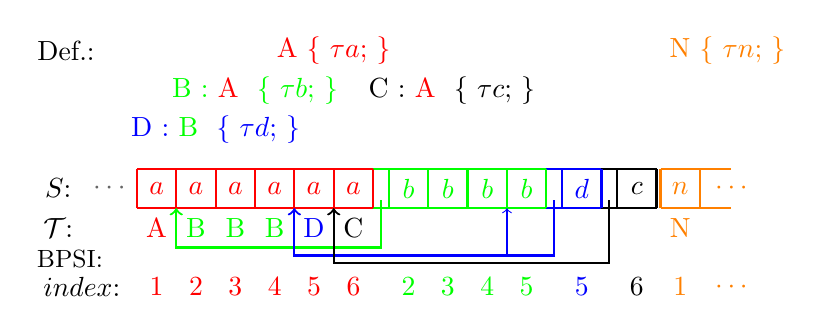
\begin{tikzpicture}
%labels
\node[draw=none] at (-1,0.25) {$S$:};
\node[draw=none] at (-1,-0.25) {$\mathcal{T}$:};
\node[draw=none] at (-0.7,-1) {$index$:};
\node[draw=none] at (-0.85,-0.65) {\small{BPSI}:};
\node[draw=none] at (-0.9,2) {Def.:};

%definitions
\node[red,draw=none] at (2.5,2) {A \{ $\tau a$; \} };
\node[green,draw=none] at (1.5,1.5) {B : {\color{red} A } \{ $\tau b$; \} };
\node[blue,draw=none] at (1,1) {D : {\color{green} B } \{ $\tau d$; \} };
\node[black,draw=none] at (4,1.5) {C : {\color{red} A } \{ $\tau c$; \} };

\node[orange,draw=none] at (7.5,2) {N \{ $\tau n$; \} };

%content
 \node[color=black!60,draw=none] at (-0.35,0.25) {$\cdots$};
 
 \node[red,draw=none] at (0.25,0.25) {${a}$};
 \node[red,draw=none] at (0.75,0.25) {${a}$};
 \node[red,draw=none] at (1.25,0.25) {${a}$};
 \node[red,draw=none] at (1.75,0.25) {${a}$};
 \node[red,draw=none] at (2.25,0.25) {${a}$};
 \node[red,draw=none] at (2.75,0.25) {${a}$};
 
 \node[green,draw=none] at (3.45,0.25) {$b$};
 \node[green,draw=none] at (3.95,0.25) {${b}$};
 \node[green,draw=none] at (4.45,0.25) {${b}$};
 \node[green,draw=none] at (4.95,0.25) {${b}$};
 
 \node[blue,draw=none] at (5.65,0.25) {${d}$};
 
 \node[black,draw=none] at (6.35,0.25) {${c}$};
 
 \node[orange,draw=none] at (6.9,0.25) {${n}$};
 \node[orange,draw=none] at (7.55,0.25) {$\cdots$};
 
%base pool index
 
 \node[red,draw=none] at (0.25,-1) {1};
 \node[red,draw=none] at (0.75,-1) {2};
 \node[red,draw=none] at (1.25,-1) {3};
 \node[red,draw=none] at (1.75,-1) {4};
 \node[red,draw=none] at (2.25,-1) {5};
 \node[red,draw=none] at (2.75,-1) {6};
 
 \node[green,draw=none] at (3.45,-1) {2};
 \node[green,draw=none] at (3.95,-1) {3};
 \node[green,draw=none] at (4.45,-1) {4};
 \node[green,draw=none] at (4.95,-1) {5};
 
 \node[blue,draw=none] at (5.65,-1) {5};
 
 \node[black,draw=none] at (6.35,-1) {6};
 
 \node[orange,draw=none] at (6.9,-1) {1};
 \node[orange,draw=none] at (7.55,-1) {$\cdots$};
 
%base pool types
 \node[red,draw=none] at (0.25,-0.25) {A};
 \node[green,draw=none] at (0.75,-0.25) {B};
 \node[green,draw=none] at (1.25,-0.25) {B};
 \node[green,draw=none] at (1.75,-0.25) {B};
 \node[blue,draw=none] at (2.25,-0.25) {D};
 
 \node[black,draw=none] at (2.75,-0.25) {C};
 
 \node[orange,draw=none] at (6.9,-0.25) {N};

%frames
 \draw[shift={(0.15,0)},thick,orange] (6.4999,0) grid [step=0.5] (7.4,0.5);

 \draw[shift={(0.6,0)},thick,black] (5.3,0) grid [step=0.5] (6,0.5);
 \draw[shift={(0.4,0)},thick,blue] (4.8,0) grid [step=0.5] (5.5,0.5);
 \draw[shift={(0.2,0)},thick,green] (2.8,0) grid [step=0.5] (5,0.5);
 \draw[thick,red] (0,0) grid [step=0.5] (3,0.5);
 
%base type indices
 \draw[thick,green,->] (3.1,0.1) -- (3.1,-0.5) -- (0.5,-0.5) -- (0.5,0);
 \draw[thick,blue,->] (5.3,0.1) -- (5.3,-0.6) -- (2,-0.6) -- (2,0);
 \draw[blue,->] (5.3,0.1) -- (5.3,-0.6) -- (4.7,-0.6) -- (4.7,0);
 \draw[thick,black,->] (6,0.1) -- (6,-0.7) -- (2.5,-0.7) -- (2.5,0);
\end{tikzpicture}
\caption{The serialization scheme used to store objects into pools.}
\end{figure}

The order in which pools are serialized is currently unrestricted.


\subsection{Pool Elements}
\label{serialization:elements}

In this section, we want to describe the serialization of individual fields using the function $\den{\_}_\tau$. The serialization of an objects takes places by serializing all its fields into the stream. In this section, we assume that the three functions defined in the last section are implicitly converted to streams using the v64 encoding. We assume further, that compound types provide a function $size: \mathcal{T} → \mathcal{I}$, which returns the number of elements stored in a given field.
Let $f$ be a field of type $t$, then $\den{f}$ is defined as\footnote{We will use C-Style hexadecimal integer literals for integers in streams.}
\begin{itemize}
 %pooled objects
 \item $\forall t \in \mathcal{U}\cup\{\textbf{string}\}. \den{f}_t = \left\{ 
   \begin{array}{l l}
     \texttt{0x00}, & f = \texttt{NULL}\\
     index(f) & else
   \end{array} \right.$
 
 %annotation -> * (v64 baseTypeName!!, v64index)
 \item $\den{f}_{\textbf{annotation}} = \left\{ 
   \begin{array}{l l}
     \texttt{0x00 0x00}, & f = \texttt{NULL}\\
     baseTypeName(f) \circ index(t) & else
   \end{array} \right.$
   \footnote{We do not want to use type IDs here, because we do not want to touch all annotation fields if we modify the type Pool.}
 
 %bool
 \item $\den{\top}_\textbf{bool} = \texttt{0xFF}$
 \item $\den{\bot}_\textbf{bool} = \texttt{0x00}$
 
 %fixed int
 \item $\forall t \in \mathcal{I}\setminus\{\textbf{v64}\}. \den{f}_t = f$
 
 %v64
 \item $\den{f}_\textbf{v64} = encode(f)$\footnote{With encode as defined in listing \ref{v64enc}.}
 
 %fixed float
 \item $\den{f}_\textbf{f32} = \den{f}_\textbf{f64} = f$\footnote{Assuming the float to be IEEE-754 encoded, which allows for an implicit bit-wise conversion to fixed sized integer.}
 
 %fixed and dependent arrays
 \item $\forall g \in \mathcal{B}, n \in \mathbb{N}^+. t = g\texttt{[}n\texttt{]} \implies \den{f} = \den{f_0}_g \circ \cdots \circ \den{f_{n-1}}_g$
 
 \item $\forall g \in \mathcal{B}, s \in \mathcal{I}, \texttt{s size}$\footnote{As stated above, size must be a field of the same declaration as f.} $. t = g\texttt{[size]} \wedge \texttt{size} > 0 \implies \den{f} = \den{f_0}_g \circ \cdots \circ \den{f_{\texttt{size}-1}}_g$\footnote{Note that this is the only case where the encoded field does not append anything to the stream.}
 
 %variable array, list and set
 \item $\forall g \in \mathcal{B}, n = size(f), t \in \{g\texttt{[]}, \texttt{set<}g\texttt{>}, \texttt{list<}g\texttt{>}\}. \den{f} = \den{n}_{v64} \circ \den{f_0}_g \circ \cdots \circ \den{f_{n-1}}_g$
 
 %map
 \item Maps are serialized from left to right by serializing the keyset and amending each key with the map structure which it points to. In case of Maps with two types, this is equal to a list of key value tuples.
 A field of type \verb/map<T,U,V>/ is serialized using a schema $ \den{size(f)} \circ \den{f.t_1} \circ \den{size(f[t_1])} \circ \den{f[t_1].u_1} \circ \den{f[t_1][u_1]} \circ \den{f[t_1].u_2} \circ \cdots \circ \den{size(f[t_2])} \circ \cdots \circ \den{f[t_n][u_m]}$. Note that we treat maps like map<T, map<U,V>>.
 
 %restrictions
 \item $\den{RESTRICTION} = \left\{ 
   \begin{array}{l l}
     \emptyset, & id = \bot\\
     \den{id}_{v64}\den{arg_1}_{string}\circ \cdots \circ \den{arg_n}_{string} & else
   \end{array} \right.$
 
 %types
 \item $\den{t}_{type} = \left\{ 
   \begin{array}{l l}
   \den{id}_{i8} \circ \den{val}_{t} & id \in [0,4] \\
   \den{id}_{i8} & id \in [5,14] \\
   15 \circ \den{i}_{v64} \circ \den{T} & t = T[i]\\
   16 \circ \den{f.nameIndex}_{v64} \circ \den{T} & t = T[f]\\
   17 \circ \den{T} & t = T[]\\
   18 \circ \den{T} & t = list<T>\\
   19 \circ \den{T} & t = set<T>\\
   20\circ \den{n}_{v64} \circ \den{T_1} \circ \cdots \circ \den{T_n} & t = map<T_i,\ldots,T_n>\\
   \den{21+reflectionPoolIndex(t)}_{v64} & t \in \mathcal{U}\\
   \end{array} \right.$
\end{itemize}
Note that \textit{id}s of restrictions and types a listed in appendix \ref{app:constants}.


\subsection{Endianness}

Files are stored in a little endian format, which is the default for common architectures.

If a client is running on a big endian machine, the endianness has to be corrected, both when reading and writing files. This can be done by changing the implementation of $\den{\_}_{i*}$- and $\den{\_}_{f*}$-translations.



\section{Deserialization}

Deserialization is mostly straight forward.

The general strategy is:
\begin{itemize}
 \item the string pool is deserialized into an array
 \item the reflection pool is deserialized using the strings array
 \item the structure of storage pools is read, pools are created and chunks of field data are copied into memory
 \item required fields are parsed using the information from the reflection pool
\end{itemize}

\subsection*{Date Example}

Let $d$ be the deserialization function -- basically the inverse function of \den{\_}.

$d(01 04 64 61  74 65 01 00  02 00 01 00  0B 01 0A 01   FF FF FF FF  FF FF FF FF  FF)$\\
$=d(01) d(04 64 61  74 65 01 00  02 00 01 00  0B 01 0A 01   FF FF FF FF  FF FF FF FF  FF)$\\
$=d(01) d(04) d(64 61  74 65 01 00  02 00 01 00  0B 01 0A 01   FF FF FF FF  FF FF FF FF  FF)$
$=d(01) d(04) d(64 61  74 65) d(01 00  02 00 01 00  0B 01 0A 01   FF FF FF FF  FF FF FF FF  FF)$
$=string[1:"date"] d(01 00  02 00 01 00  0B 01 0A 01   FF FF FF FF  FF FF FF FF  FF)$
$=string[1:"date"] d(01) d(00) d(02) d(00) d(01) d(00  0B 01 0A 01   FF FF FF FF  FF FF FF FF  FF)$
$=string[1:"date"] date[T:date[\_] 1:\_ 2:\_ d(00  0B 01 0A 01   FF FF FF FF  FF FF FF FF  FF)$
$=string[1:"date"] date[T:date[d(00  0B 01)] 1:\_ 2:\_ d(0A 01   FF FF FF FF  FF FF FF FF  FF)$
$=string[1:"date"] date[T:date[v64 date] 1:\_ 2:\_ d(0A 01   FF FF FF FF  FF FF FF FF  FF)$
$=string[1:"date"] date[T:date[v64 date] 1:\_ 2:\_ d(01   FF FF FF FF  FF FF FF FF  FF)]$
$=string[1:"date"] date[T:date[v64 date] 1:[1] 2:[-1]]$